% Chapter 2

\chapter{Scope} % Main chapter title
\label{Chapter2} % For referencing the chapter elsewhere, use \ref{Chapter2} 

This chapter presents the scope of the thesis. Apart of literature review, the
main work on this research are the work on the models implementation for remote
attestation and the analysis of the model's performance. Section
\ref{sec:implementation} presents the scope of implementation. Section
\ref{sec:analysis}) discusses the scope of the analysis.

\section{Implementation}
\label{sec:implementation}

\begin{figure}[htbp]
\centerline{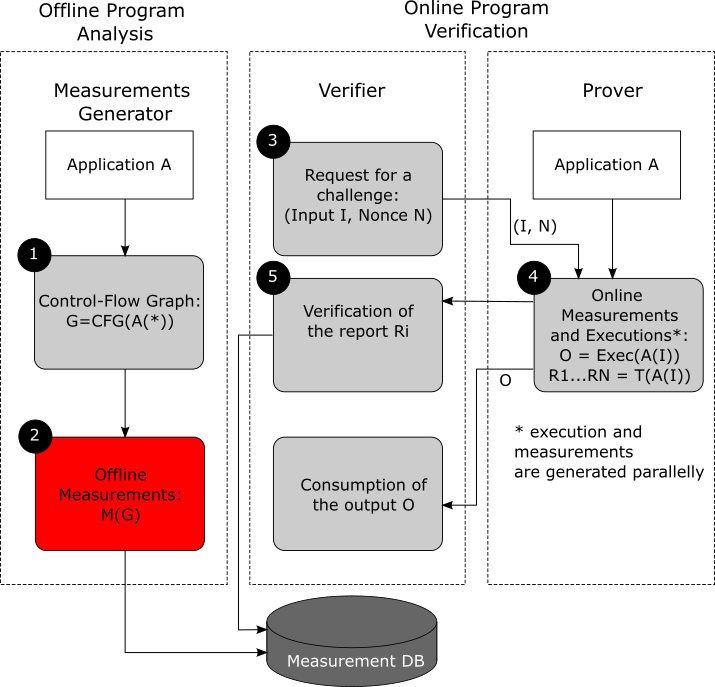
\includegraphics[scale=.5]{Figures/02/scarr-system-overview.png}}
\caption{ScaRR System Overview}
\label{fig:scarr-system-overview}
\end{figure}

In Chapter \ref{Chapter1}, we presented different runtime remote attestation
approaches. In learning the different models of runtime remote attestation, we
implemented one of the model: ScaRR Control-Flow Model
\cite{toffaliniScaRRScalableRuntime2019}. Specifically we write a tool to
extract offline measurement using the ScaRR control-flow model. ScaRR system as
shown in figure \ref{fig:scarr-system-overview}, consists of offline program
analysis and online program verification. This thesis will focus on the offline
program analysis part, specifically on the offline measurements generator as
shown in the red box in the figure \ref{fig:scarr-system-overview}.

The offline measurement is information that will be used in runtime remote
attesttion. We write the offline measurement as LLVM passes using LLVM 13.0.0.
We designed the algorithm based on the description in the original paper. 


We tested the model implementation using different programs that is written in
C. Since the LLVM pass is running control from graph extraction against the
intermediate representation, we should get consistent result on any programming
language that compiles to IR. 


\section{Analysis}
\label{sec:analysis}

We analyze the control-flow model extracted against different programs with
various size and complexities. In this thesis, we are only analyzing program
written in C. The analysis is comparing the program size with different
measurements defined by the ScaRR control-flow model. We present the detail of
the methodology in chapter \ref{Chapter4} and show the analysis result in
chapter \ref{Chapter5}.